\documentclass[tikz,border=2]{standalone}
\usetikzlibrary{shadows,arrows,shapes,positioning,calc,backgrounds,fit}
\newcommand{\vanish}[1]{}
\usepackage{colortbl}
\usepackage{array}
\usepackage{amssymb}
\usepackage{multirow}
\newcommand{\shaded}[1]{\cellcolor{black!20}{#1}}
\newcommand{\calc}[1]{\mbox{$\mathcal{C}_{#1}$}}
\pdfpageattr {/Group << /S /Transparency /I true /CS /DeviceRGB>>}
\newcommand{\mathtttt}{}
% Define the layers to draw the diagram
%
\begin{document}
%% \pgfdeclarelayer{bg}
%% \pgfdeclarelayer{fg}
%% \pgfsetlayers{bg,main,fg}
\newcommand{\ttbig}{\mathtt{big}}
\newcommand{\ttsmall}{\mathtt{small}}
\newcommand{\ttwifi}{\mathtt{wifi}}
\newcommand{\ttcab}{\mathtt{cab}}
%
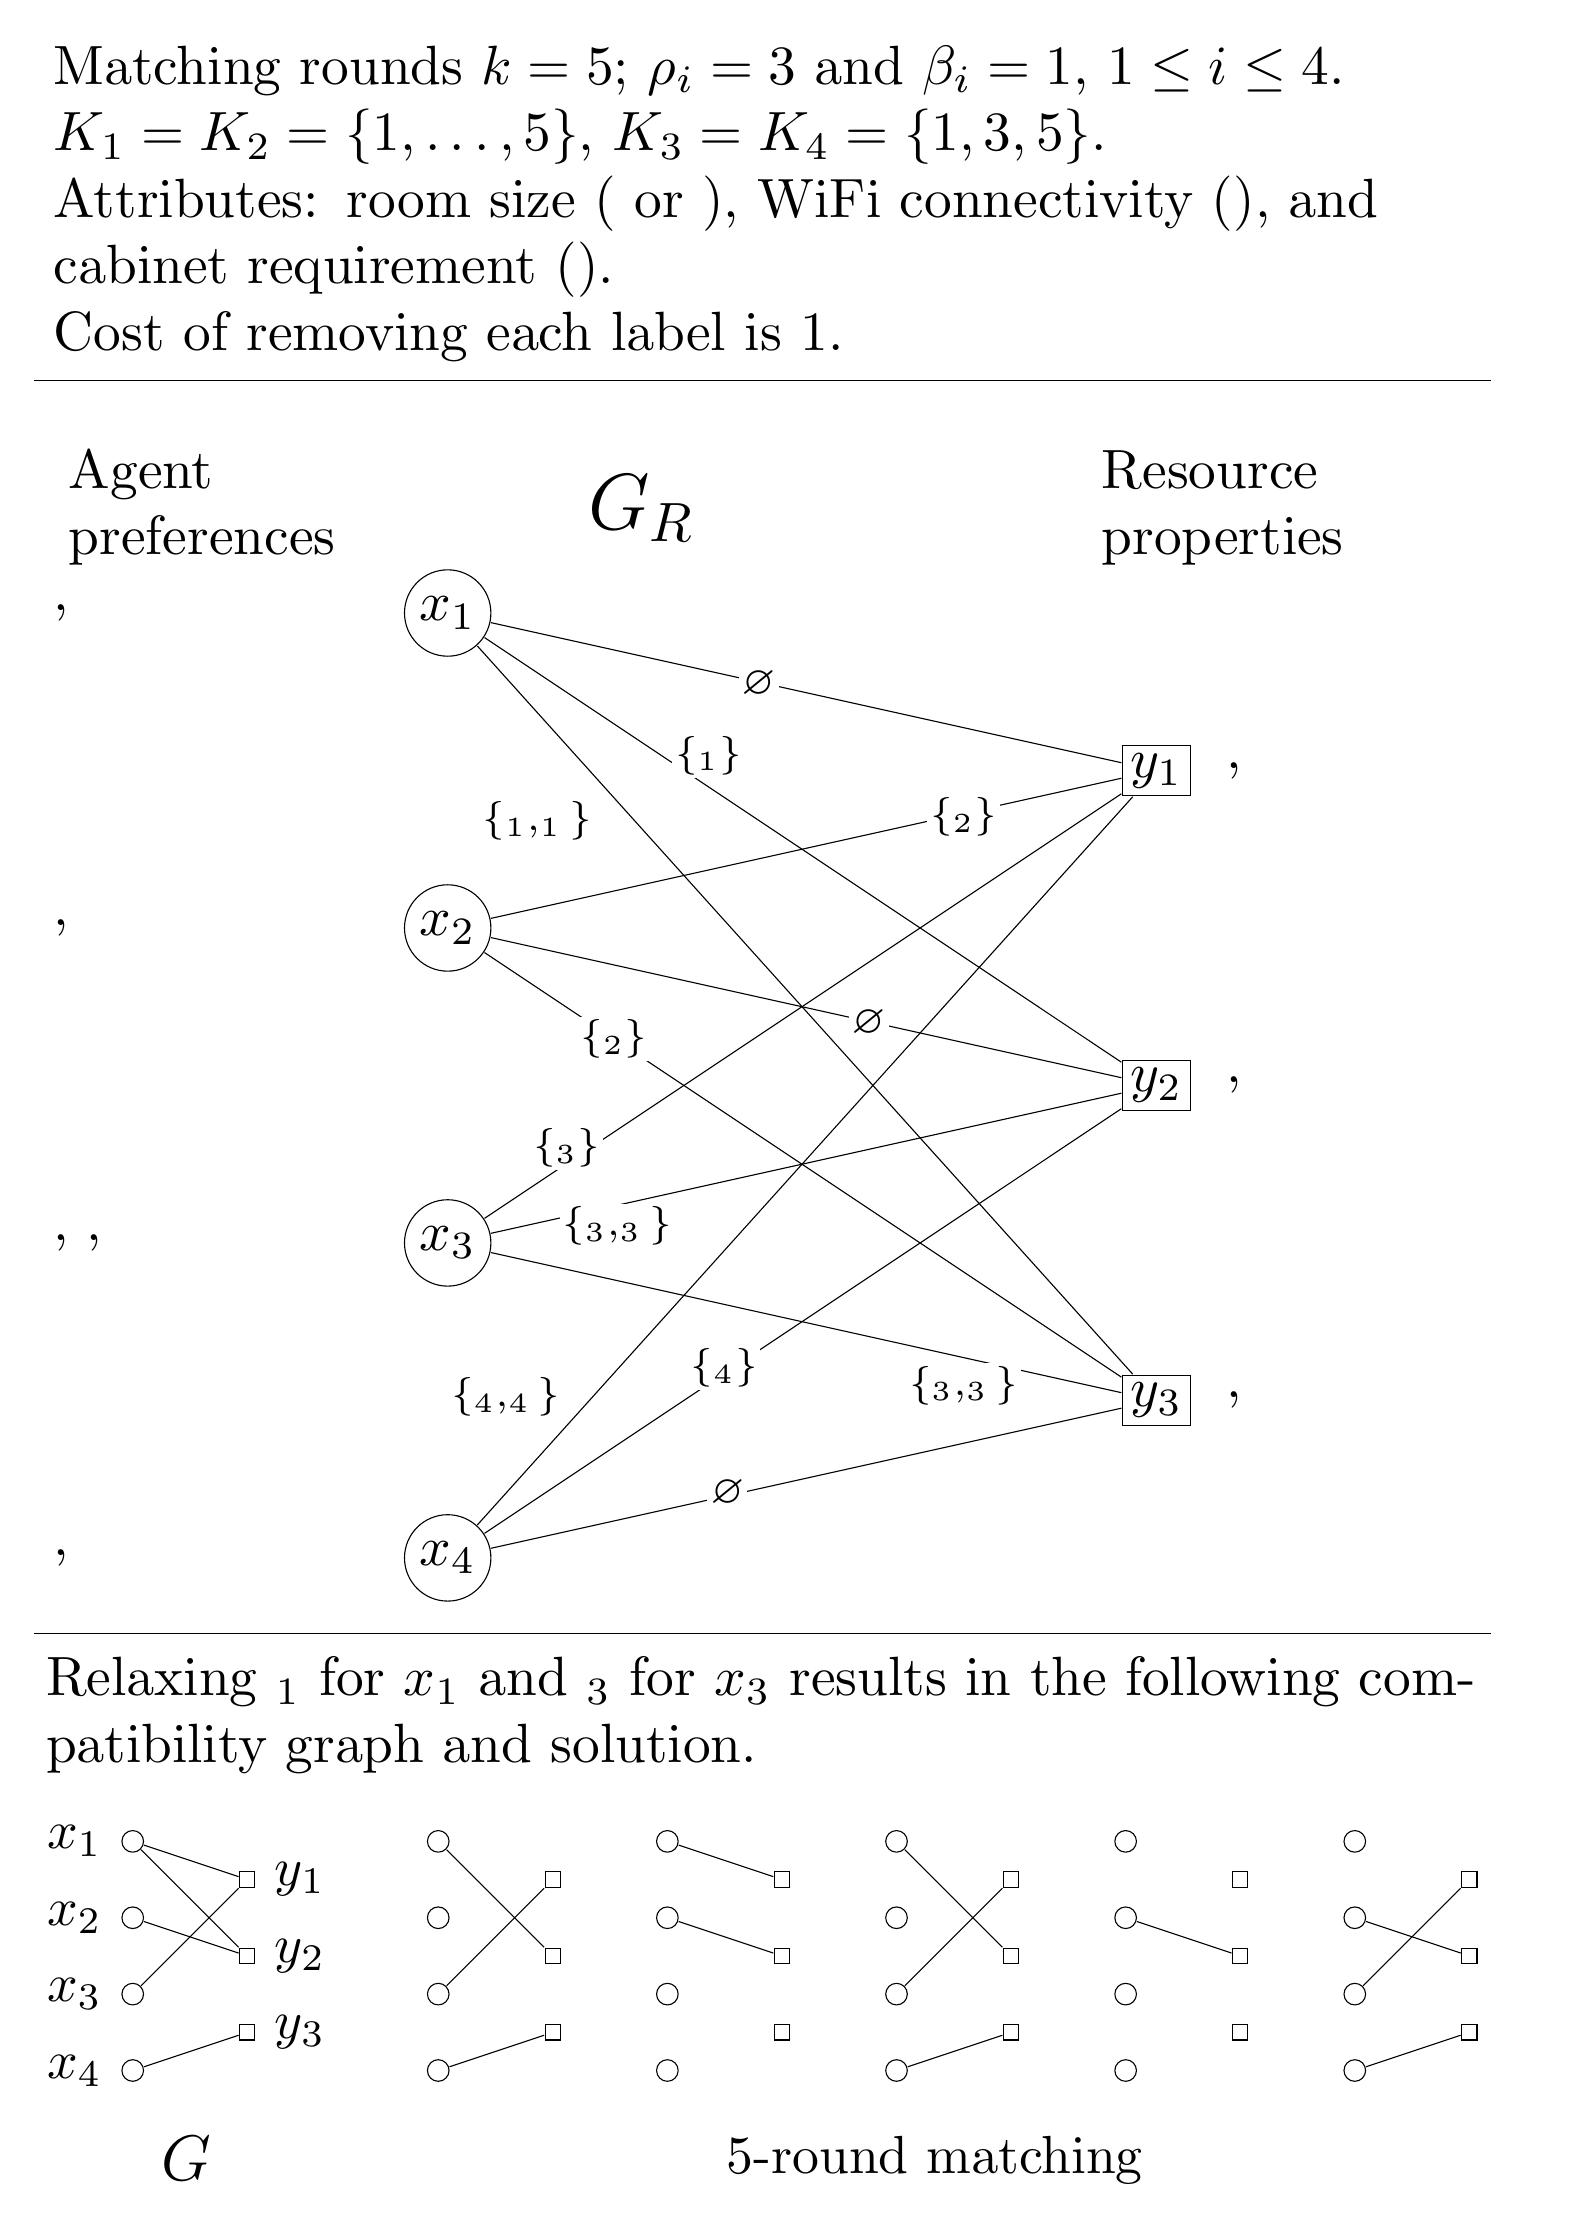
\begin{tikzpicture}
[scale=2,node distance=.5cm, transform shape,
    agent/.style={draw,shape=circle,inner sep=.5mm},
    res/.style={shape=rectangle,draw,inner sep=.5mm},
    lab/.style={fill=white,font=\scriptsize,inner sep=.5pt},
    prop/.style={text width=2cm},
myedge/.style={>=latex', shorten >=.0pt, shorten <=.0pt,semithick}]
%%%%%%%%%%
%%%%% The underlying graph with preferences and properties
\begin{scope}
    \node[text width=9cm] (desc) {Matching rounds~$k=5$; $\rho_i=3$ and
        $\beta_i=1$, $1\le i\le 4$. \\
        $K_1=K_2=\{1,\ldots,5\}$, $K_3=K_4=\{1,3,5\}$.\\
        Attributes: room size ($\ttbig$ or $\ttsmall$), WiFi connectivity
        ($\ttwifi$), and cabinet requirement ($\ttcab$).\\
    Cost of removing each label is $1$.
};
    \draw (desc.south west) -- (desc.south east);
\end{scope}
%%
\begin{scope}[shift={(-2,-2.6)}]
%% nodes
\node (x1) [agent] at (0,0)  {$x_1$};
\node (x2) [agent] at (0,-2) {$x_2$};
\node (x3) [agent] at (0,-4) {$x_3$};
\node (x4) [agent] at (0,-6) {$x_4$};
\node (y1) [res] at (4.5,-1) {$y_1$};
\node (y2) [res] at (4.5,-3) {$y_2$};
\node (y3) [res] at (4.5,-5) {$y_3$};
%% agent preferences
\node (px1) [prop,left=of x1,shift={(.4,0)}] {$\ttbig$, $\ttwifi$};
\node (px2) [prop,left=of x2,shift={(.4,0)}] {$\ttsmall,\ttwifi$};
\node (px3) [prop,left=of x3,shift={(.4,0)}] {$\ttbig$, $\ttwifi$, $\ttcab$};
\node (px4) [prop,left=of x4,shift={(.4,0)}] {$\ttsmall$, $\ttcab$};
\node (tap) [above=of px1, text width=1.8cm, shift={(0,-.5)}] {Agent \\preferences};
\node (Gr) [right=of tap,shift={(.75,0)}] {\Large $G_R$};
%% resource properties
\node (py1) [right=of y1,shift={(-.4,0)}] {$\ttbig$, $\ttwifi$};
\node (py2) [right=of y2,shift={(-.4,0)}] {$\ttsmall$, $\ttwifi$};
\node (py3) [right=of y3,shift={(-.4,0)}] {$\ttsmall$, $\ttcab$};
\node (trp) [text width=1.8cm] at (py1|-tap) {Resource \\properties};
%% edges
\draw (x1) -- node[lab,shift={(-.3,.05)}]{$\varnothing$} (y1); 
\draw (x1) -- node[lab,shift={(-.6,.6)}]{$\{\ttbig_1\}$} (y2); 
\draw (x1) -- node[lab,shift={(-1.7,1.2)}]{$\{\ttbig_1, \ttwifi_1\}$} (y3); 
\draw (x2) -- node[lab,shift={(1,.2)}]{$\{\ttsmall_2\}$} (y1); 
\draw (x2) -- node[lab,shift={(.4,-.1)}]{$\varnothing$} (y2); 
\draw (x2) -- node[lab,shift={(-1.2,.8)}]{$\{\ttwifi_2\}$} (y3); 
\draw (x3) -- node[lab,shift={(-1.5,.-.9)}]{$\{\ttcab_3\}$} (y1); 
\draw (x3) -- node[lab,shift={(-1.2,-.4)}]{$\{\ttbig_3,\ttcab_3\}$} (y2); 
\draw (x3) -- node[lab,shift={(1,-.4)}]{$\{\ttbig_3,\ttwifi_3\}$} (y3); 
\draw (x4) -- node[lab,shift={(-1.9,.-1.5)}]{$\{\ttsmall_4,\ttcab_4\}$} (y1); 
\draw (x4) -- node[lab,shift={(-.5,.-.3)}]{$\{\ttcab_4\}$} (y2); 
\draw (x4) -- node[lab,shift={(-.5,.-.1)}]{$\varnothing$} (y3); 
\node (anc) at ($(x4.south)+(0,-.2)$) {};
\draw (desc.south west|-anc) -- (desc.south east|-anc);
\end{scope}
%%
\begin{scope}[shift={(0.2,-9.6)}]
    \node [text width=9.5cm] {Relaxing $\ttbig_1$ for $x_1$ and 
        $\ttcab_3$ for $x_3$ results in the following
compatibility graph and solution.};
\end{scope}
%% Gc
\begin{scope}[shift={(-4,-10.4)},scale=.97]
\begin{scope}[shift={(0,0)},local bounding box=Gc]
\node (x1) [agent, label=left:$x_1$] at (0,0)  {};
\node (x2) [agent, label=left:$x_2$] at (0,-.5) {};
\node (x3) [agent, label=left:$x_3$] at (0,-1) {};
\node (x4) [agent, label=left:$x_4$] at (0,-1.5) {};
\node (y1) [res, label=right:$y_1$] at (.75,-.25) {};
\node (y2) [res, label=right:$y_2$] at (.75,-.75) {};
\node (y3) [res, label=right:$y_3$] at (.75,-1.25) {};
\draw (x1) -- (y1);
\draw (x1) -- (y2);
\draw (x2) -- (y2);
\draw (x3) -- (y1);
\draw (x4) -- (y3);
\node [below=of y3,shift={(-.4,0)}] {\large$G$};
%%\draw (1.5,.1) -- +(0,-1.7);
\end{scope}
%% matching 1
\begin{scope}[shift={(2,0)}]
\node (x1) [agent] at (0,0)  {};
\node (x2) [agent] at (0,-.5) {};
\node (x3) [agent] at (0,-1) {};
\node (x4) [agent] at (0,-1.5) {};
\node (y1) [res] at (.75,-.25) {};
\node (y2) [res] at (.75,-.75) {};
\node (y3) [res] at (.75,-1.25) {};
\draw (x1) -- (y2);
\draw (x3) -- (y1);
\draw (x4) -- (y3);
\end{scope}
%% matching 2
\begin{scope}[shift={(3.5,0)}]
\node (x1) [agent] at (0,0)  {};
\node (x2) [agent] at (0,-.5) {};
\node (x3) [agent] at (0,-1) {};
\node (x4) [agent] at (0,-1.5) {};
\node (y1) [res] at (.75,-.25) {};
\node (y2) [res] at (.75,-.75) {};
\node (y3) [res] at (.75,-1.25) {};
\draw (x1) -- (y1);
\draw (x2) -- (y2);
\end{scope}
%% matching 3
\begin{scope}[shift={(5,0)}]
\node (x1) [agent] at (0,0)  {};
\node (x2) [agent] at (0,-.5) {};
\node (x3) [agent] at (0,-1) {};
\node (x4) [agent] at (0,-1.5) {};
\node (y1) [res] at (.75,-.25) {};
\node (y2) [res] at (.75,-.75) {};
\node (y3) [res] at (.75,-1.25) {};
\draw (x1) -- (y2);
\draw (x3) -- (y1);
\draw (x4) -- (y3);
\end{scope}
%% matching 4
\begin{scope}[shift={(6.5,0)}]
\node (x1) [agent] at (0,0)  {};
\node (x2) [agent] at (0,-.5) {};
\node (x3) [agent] at (0,-1) {};
\node (x4) [agent] at (0,-1.5) {};
\node (y1) [res] at (.75,-.25) {};
\node (y2) [res] at (.75,-.75) {};
\node (y3) [res] at (.75,-1.25) {};
\draw (x2) -- (y2);
\end{scope}
%% matching 5
\begin{scope}[shift={(8,0)}]
\node (x1) [agent] at (0,0)  {};
\node (x2) [agent] at (0,-.5) {};
\node (x3) [agent] at (0,-1) {};
\node (x4) [agent] at (0,-1.5) {};
\node (y1) [res] at (.75,-.25) {};
\node (y2) [res] at (.75,-.75) {};
\node (y3) [res] at (.75,-1.25) {};
\draw (x2) -- (y2);
\draw (x3) -- (y1);
\draw (x4) -- (y3);
\node [below=of y3,shift={(-3.5,0)}] {$5$-round matching};
\end{scope}
\end{scope}
\end{tikzpicture}
\end{document}
